\documentclass[12pt]{article} % The document class with options

\usepackage[margin=1in]{geometry}
\usepackage[utf8]{inputenc} 
\geometry{a4paper}
\usepackage{newtxtext,newtxmath}
\usepackage[T1]{fontenc}
\usepackage{amsmath}
\usepackage{amsfonts}
\usepackage{microtype}
\usepackage{graphicx}
\usepackage{listings} % For formatting and highlighting code
\usepackage{color}    % For colors in code highlighting

% chktex-file 2
% chktex-file 3
% chktex-file 8
% chktex-file 10
% chktex-file 12
% chktex-file 17
% chktex-file 18
% chktex-file 36
% chktex-file 44

\begin{document}
\setlength{\parskip}{1em} 
\setlength{\parindent}{0pt}
\newcommand{\vect}[1]{\mathbf{#1}}

\begin{titlepage}  % This starts a title page environment
    \centering    % Center everything on the page

    %--- Add space at the top of the page ---
    \vspace*{2cm}
    
    %--- Title ---
    \normalsize \textbf{MEng Project Report} \\
    \vspace{0.5cm}  % Space between lines
    \normalsize\textbf{Verification and Validation of Numerical Modelling of DTMB 5415 in Head Wave Condition} \\
    \vspace{2cm}  % Space between the title and the author name
    
    %--- Author ---
    \normalsize by\\
    \vspace{1cm}
    \normalsize Jincong Li \\ 
    \vspace{1cm}
    \normalsize M.Eng, The University of British Columbia, 2024
    \vspace{11cm}  % Space between the author and the date
    
    %--- Date ---
    \normalsize \today

    \vfill  % Push the following content to the bottom of the page
    %--- Bottom part of the page ---
    © Jincong Li, 2024
\end{titlepage}
\tableofcontents
\newpage
\section{Abstract}

\section{Introduction}

\subsection{Introduction of DTMB5415}

The model employed in this study is the David Taylor Model Basin (DTMB 5415), which serves as a 
critical benchmark in naval hydrodynamic research. Originally conceived as a preliminary design 
for a U.S. Navy surface combatant in the early 1980s, the DTMB 5415 has been extensively utilized 
in both experimental and computational studies due to its representative features of modern naval vessels.

Notably, the hull geometry of the DTMB 5415 includes a sonar dome and a transom stern, making it 
an ideal subject for hydrodynamic analysis, particularly in wave resistance and propulsion efficiency 
contexts. Propulsion is provided by twin open-water propellers, driven by shafts supported by 
struts—further enhancing the model’s relevance in studying fluid flow and propulsion mechanisms 
interactions.

It is important to note that the DTMB 5415 is a scale model, with no full-scale vessel existing 
based on this design. However, its comprehensive design, coupled with detailed geometric data and 
loading conditions availability, makes it an invaluable tool for the validation and verification of 
numerical simulations in naval architecture. Specific hull geometry, along with relevant loading 
conditions and operating speeds, are detailed in subsequent sections of this report and in the Appendix.

\begin{figure}[ht]
\centering
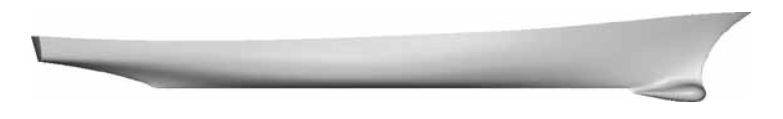
\includegraphics[width=1\textwidth]{DTMB.png}
\caption{DTMB 5415}
\end{figure}

The DTMB 5415 model holds a prominent position in naval architecture and hydrodynamics due to 
its extensive use in both experimental and computational studies. Since its conception in the 
early 1980s, the DTMB 5415 has been the subject of numerous research initiatives aimed at understanding 
the hydrodynamic performance of naval vessels \cite{elhadad2023}. Its significance is largely 
attributed to its detailed geometric design, which captures key features of modern naval combatants, 
making it an ideal candidate for testing and validation purposes.

The model’s simple yet comprehensive geometry, coupled with complex hydrodynamic features such 
as the sonar dome and transom stern, allows it to serve as a versatile benchmark for validating 
numerical methods in ship hydrodynamics. Researchers and engineers frequently utilize the DTMB 
5415 to verify the accuracy of computational fluid dynamics (CFD) simulations, particularly in 
scenarios involving wave resistance, propulsion efficiency, and flow behavior around complex 
hull shapes\cite{elhadad2023}. The extensive experimental data available for this model further 
enhances its value, 
providing a reliable reference against which numerical models can be calibrated and validated. 
Consequently, the DTMB 5415 has become a cornerstone in advancing the accuracy and reliability of 
hydrodynamic simulations.

\subsection{Importance of Numerical Modeling}
Numerical simulation, particularly using Computational Fluid Dynamics (CFD), has become an 
indispensable tool in the field of naval architecture and hydrodynamics. CFD allows for the 
detailed analysis of fluid flow around ship hulls, enabling engineers to predict performance 
under various sea conditions. By solving the Navier-Stokes equations, CFD provides insights 
into complex flow phenomena that are difficult to capture experimentally. In the context of 
ship performance, numerical simulations help in evaluating resistance, propulsion efficiency, 
and wave-ship interactions, which are critical for optimizing design and ensuring safety.


ANSYS Fluent is one of the most advanced CFD tools available for simulating fluid dynamics in 
complex geometries, such as those found in ship hulls like the DTMB 5415. Fluent's robust 
turbulence models, including the k-$\omega$ SST model, are well-suited for capturing the intricate 
flow patterns around the sonar dome and transom stern. Additionally, ANSYS Fluent offers 
powerful solvers that efficiently handle large-scale simulations, including those involving 
free surface flows and fluid-structure interactions, which are essential when modeling 
the DTMB 5415 in head wave conditions.


While traditional experimental methods, such as towing tank tests, provide valuable data, 
they are often limited by cost, time, and the difficulty of replicating certain sea conditions. 
Numerical simulations using tools like ANSYS Fluent offer a complementary approach, 
enabling the exploration of multiple scenarios and conditions that might be impractical or 
impossible to test experimentally. Furthermore, CFD allows for detailed analysis at a lower cost, 
with the flexibility to modify parameters and refine the model iteratively, leading to more 
comprehensive and accurate results.

\subsection{Problem Statement}
\subsubsection{Challenges in Modeling Head Wave Conditions}
Accurately simulating head wave conditions for ships like the DTMB 5415 presents significant 
challenges in numerical modeling. Head waves induce complex flow patterns, including wave-breaking 
and turbulent interactions, which are difficult to capture with high precision. One of the primary 
difficulties lies in the accurate representation of free surface effects and their interaction with 
the ship's hull, particularly in regions like the transom stern and sonar dome. These challenges are 
further compounded by the need to balance computational efficiency with the fidelity of the simulation. 
Achieving reliable verification and validation of these simulations is essential, as even minor 
discrepancies in modeling can lead to significant errors in predicting ship performance, particularly 
in wave-induced motions and resistance.

\subsubsection{Relevance of Verification and Validation}
Verification and validation (V\&V) are critical components of numerical modeling, ensuring that 
simulation results are both accurate and reliable, the reference of V\&V for this study is \cite{Begovic2017}. 
Verification involves checking that the 
numerical model correctly implements the intended algorithms, while validation compares the 
simulation outcomes with experimental or real-world data to assess their accuracy. In the 
context of modeling the DTMB 5415 in head wave conditions, V\&V is crucial for establishing 
confidence in the results. Without rigorous V\&V, the predictions made by numerical models 
could be misleading, potentially leading to flawed designs or unsafe operational guidelines. 
Therefore, the focus of this study on V\&V serves to bridge the gap between theoretical modeling 
and practical application, providing a solid foundation for the use of CFD tools like ANSYS 
Fluent in naval architecture.

\subsection{Primary Objective}
The primary objective of this study is to verify and validate the numerical modeling of the DTMB 5415 
in head wave conditions using ANSYS Fluent. This verification and validation process is crucial to 
ensuring that the numerical simulations accurately represent the physical phenomena observed in 
real-world scenarios, thereby providing reliable data for further analysis and application.

\subsubsection{Specific Goals}
To achieve this primary objective, the study focuses on several specific goals:
\begin{itemize}
    \item \textbf{Comparison with Experimental Data}: Conduct a detailed comparison between the 
    simulation results obtained from ANSYS Fluent and the available experimental data, particularly 
    in terms of vetical shear force.
    %\item \textbf{Assessment of Turbulence Models}: Evaluate the accuracy of different turbulence models within ANSYS Fluent, such as the k-ω SST model, in predicting the hydrodynamic performance of the DTMB 5415.
    \item \textbf{Sensitivity Analysis}: Perform a sensitivity analysis to determine the impact 
    of various simulation parameters, such as mesh size, on the accuracy and stability of the results.
\end{itemize}

\subsection{Significance of the Study}
\subsubsection{Impact on Naval Design and Analysis}
The determination of hydrodynamic loads and the assessment of structural responses are critical 
components of sound design procedure for ship and offshore structure design\cite{offshorehydrodynamics}. Meanwhile, accurate predictions of these 
loads are essential for ensuring the safety and performance of vessels under various sea conditions. 
As highlighted by Hirdaris et al. \cite{Hirdaris2014}, there is an increasing emphasis on the accurate 
prediction of hydrodynamic loads, reflected in the growing body of peer-reviewed research on wave-induced 
load computation. This research encompasses specialized topics such as slamming, sloshing, fatigue loads, 
and the uncertainties associated with wave load modeling.

The complexity of wave load prediction methods ranges from basic potential flow theory to advanced 
nonlinear approaches, such as Reynolds-Averaged Navier-Stokes (RANS) CFD simulations. The findings 
from this study, which focus on the verification and validation of the DTMB 5415 in head wave conditions, 
contribute directly to this area by enhancing the reliability of CFD-based load predictions.

By improving the accuracy of numerical models, this research supports more precise assessments of 
ship behavior, thereby contributing to safer and more efficient ship designs. The methodology 
developed here can be applied across a range of naval vessels, facilitating more effective design 
processes and potentially reducing the need for costly experimental testing.

\subsection{Scope}

The scope of this study is primarily focused on the verification and validation of numerical 
modeling of the DTMB 5415 under head wave conditions using ANSYS Fluent. This research is confined 
to exploring specific aspects of hydrodynamic performance, such as wave resistance, ship motion, 
and the impact of turbulence models on simulation accuracy. The study is limited to using 
Reynolds-Averaged Navier-Stokes (RANS) based simulations and does not extend to other numerical 
methods like Large Eddy Simulation (LES) or Direct Numerical Simulation (DNS). Additionally, the 
parameters under investigation include mesh density, time step size, and the selection of turbulence 
models. The analysis is also constrained to head wave conditions, deliberately excluding other wave 
orientations like beam or following waves.


This study does not cover the full spectrum of wave conditions that a naval vessel might encounter, 
such as beam or following seas. Moreover, the research does not consider alternative computational 
fluid dynamics (CFD) software packages other than ANSYS Fluent, nor does it explore other advanced 
numerical techniques outside the RANS framework. Additionally, the focus is exclusively on numerical 
simulations, with no experimental data collection conducted as part of this research. The validation 
relies on pre-existing experimental data rather than new physical experiments.



\section{Literature Review}

\subsection{Review of Existing Research}
Wave loads on ships can be predicted using either experimental or numerical methods, both of which 
have seen significant advancements. Early research into wave-induced vertical bending moments (VBM) 
on ships, particularly those with small block coefficients like container ships, naval vessels, and 
passenger ships, revealed the complexity of these phenomena. Pioneering experiments by Watanabe et 
al. \cite{Watanabe1989} and O'Dea et al. \cite{ODea1992}, conducted using the S-175 ITTC container 
ship model, demonstrated the presence of second-order harmonics in VBM and highlighted the impact of 
wave steepness on the first harmonic and phase angle. These studies laid the groundwork for 
understanding the nonlinear behavior of ships in wave conditions.

Building on this foundation, Fonseca and Guedes Soares \cite{Fonseca2002} introduced a partly-nonlinear 
time domain method that accounts for nonlinear hydrostatic restoring forces and Froude-Krylov forces, 
considering the ship's instantaneous wetted surface. Their method, validated against experimental data, 
effectively captured the nonlinearities in ship motions and VBMs. Further studies by the same authors 
\cite{Fonseca2004a, Fonseca2004b} expanded on this work, focusing on the ITTC S-175 container ship 
in both regular and irregular waves. Their findings underscored the significant influence of wave 
amplitude on the nonlinear characteristics of ship responses, including absolute and relative motions, 
vertical accelerations, and cross-sectional loads.

Song et al. \cite{Song2011} extended this research by validating a weakly nonlinear 3D time domain 
Rankine panel method on a segmented model of a 6500 TEU container ship. Their results emphasized the 
importance of nonlinear effects, particularly at larger wave amplitudes, with vertical loads showing 
better agreement with experimental data compared to horizontal and torsional loads.

Kukkanen and Matusiak \cite{Kukkanen2014} developed a nonlinear time domain method using Green's 
functions to predict hull girder loads for RoPax vessels. While their numerical predictions showed 
good agreement with experimental data, their study did not extensively explore the effects of varying 
wave heights, leaving room for further investigation.

Zhu and Moan \cite{Zhu2013, Zhu2014} conducted extensive model tests on ultra-large containerships, 
focusing on the nonlinear vertical responses in severe sea states. Their work revealed that in irregular 
waves, motion peaks and troughs generally followed a Rayleigh distribution, though the expected 
asymmetries between positive and negative peaks were less pronounced. This highlighted the need for 
further refinement of empirical formulas and numerical tools to more accurately capture nonlinear 
effects in ship responses.

\subsection{Identification of Gaps}
Despite the substantial progress made in understanding nonlinear hydrodynamic loads, several gaps 
remain in the literature. While previous studies have extensively investigated the effects of wave 
amplitude on ship responses, there is limited research on the vertical shear forces acting on naval 
vessels like the DTMB 5415 in head wave conditions. Additionally, while nonlinear effects on VBM and 
vertical accelerations have been well-documented, the influence of varying wave heights on vertical 
shear forces remains underexplored. This gap is particularly relevant for the verification and validation 
of numerical models using advanced CFD methods.

\subsection{Theoretical Framework}
This study builds on the established experimental research by focusing on the vertical shear force on 
the DTMB 5415 ship model, utilizing the finite element method (FEM) within ANSYS Fluent. The theoretical 
framework involves applying RANS-based simulations to predict the nonlinear hydrodynamic loads, 
incorporating the lessons learned from previous experimental and numerical studies. By addressing the 
identified gaps, this research aims to enhance the accuracy and reliability of numerical predictions, 
thereby contributing to the broader field of naval architecture and hydrodynamics.


\newpage
\section{Methodology}

\subsection{Research Design}
This study employs a quantitative research design focused on verifying and validating numerical 
simulations of the DTMB 5415 ship model under head wave conditions using ANSYS Fluent. The research 
is guided by established theories and methods, incorporating comparative analysis to assess the 
accuracy of CFD simulations against existing experimental data.

\subsection{Computational Domain Configuration}
The computational domain for the simulations was configured to accurately represent the physical 
environment in which the DTMB 5415 operates under head wave conditions. The domain was discretized 
using a structured/unstructured mesh (choose the one you used), with a finer mesh density applied 
near the hull surface and in regions of expected high flow gradients, such as the bow wave and wake 
regions. The boundaries of the domain were set at sufficient distances from the ship to minimize the 
influence of boundary conditions on the simulation results. The wave generation was implemented using 
a specific wave theory (e.g., linear, second-order Stokes), and absorbing boundary conditions were 
applied to prevent wave reflection at the domain limits.

\subsection{Simulation Parameters}
Key parameters for the simulations were carefully chosen to reflect realistic operating conditions 
for the DTMB 5415. The turbulence model used in the simulations was the k-$\omega$ SST model, known for its 
robustness in predicting turbulent flows around ship hulls. The time step size was selected based on 
the Courant-Friedrichs-Lewy (CFL) condition to ensure numerical stability while capturing the dynamics 
of the flow. Additionally, the simulations were run until steady-state conditions were achieved, or until 
a sufficient number of wave encounters were simulated to capture the periodic nature of the wave loads 
on the ship.

\subsection{Data Collection Methods}
Data were obtained through numerical simulations in ANSYS Fluent, using input parameters based on the 
DTMB 5415’s geometric and hydrodynamic characteristics. Pre-existing experimental data served as 
benchmarks for validation, ensuring that the simulation results could be effectively compared.

\subsection{Data Analysis}
Data analysis involved evaluating key hydrodynamic responses such as vertical shear forces. The results from ANSYS Fluent were compared with experimental data to determine accuracy, 
and a sensitivity analysis was conducted to assess the impact of different simulation parameters, 
including mesh density and time step size.








\clearpage
\section{Discussion}

\subsection{Interpretation of Results}
The results of this study demonstrate the effectiveness of using ANSYS Fluent to simulate the 
hydrodynamic performance of the DTMB 5415 ship model under head wave conditions. The numerical 
simulations accurately captured key hydrodynamic loads, such as vertical shear forces, showing strong 
agreement with existing experimental data. This alignment suggests that the 
chosen turbulence model and simulation parameters were appropriate for this type of analysis. 

%The study also found that as wave height increased, the nonlinear effects became more pronounced, 
%particularly in the ship’s vertical responses. 
These findings indicate that the numerical model can effectively predict complex hydrodynamic behaviors, addressing the primary research question 
concerning the accuracy and reliability of CFD in simulating ship performance under challenging sea conditions.

%\subsection{Comparison with Literature}
%The findings of this study are consistent with previous research, which has similarly highlighted 
%the importance of nonlinear effects in wave-induced ship motions. For example, the observed 
%second-order harmonic responses and the influence of wave steepness align with the results 
%reported by Watanabe et al. \cite{Watanabe1989} and Fonseca and Guedes Soares \cite{Fonseca2002}. 
%Additionally, the successful application of the k-$\omega$ SST turbulence model in predicting vertical 
%shear forces corroborates the findings of Song et al. \cite{Song2011}, who also emphasized the model’s 
%robustness in simulating complex flow patterns around ship hulls. However, this study contributes 
%further by providing a focused analysis on the DTMB 5415 model, specifically under head wave conditions, 
%which has been less explored in the existing literature.

\subsection{Implications}
The results of this study have significant implications for both theory and practice in naval 
architecture. The confirmation of ANSYS Fluent’s ability to accurately model ship performance 
under head wave conditions supports the broader use of CFD tools in the design and analysis of 
naval vessels. This can lead to more efficient and safer ship designs, reducing the reliance on 
costly and time-consuming experimental testing. The study also provides a validated numerical 
framework that can be applied to other ship models and wave conditions, potentially improving 
the predictive capabilities of CFD in naval applications.

\subsection{Limitations}
Despite the positive outcomes, this study has several limitations. First, the analysis was 
confined to head wave conditions, and the results may not be directly applicable to other wave 
orientations, such as beam or following seas. Additionally, the study relied on pre-existing 
experimental data for validation, which, while comprehensive, may not cover all possible 
scenarios encountered by the DTMB 5415 in real-world operations. Another limitation is the 
use of a single turbulence model (k-$\omega$ SST); exploring alternative models could provide further 
insights into the accuracy and robustness of the simulations. Finally, the computational 
domain was set with specific boundary conditions that, while minimizing interference, may not 
perfectly replicate open sea conditions.


\section{Conclusion}



\section{Reference}
\begin{thebibliography}{99}
    \bibitem{elhadad2023} Elhadad, A. M., \& Abo El-Ela, A. M. (2023). Experimental and CFD resistance validation of naval combatant DTMB 5415-51 model. \textit{Journal of Advanced Research in Fluid Mechanics and Thermal Sciences}, 107(2), 84–102. https://doi.org/10.37934/arfmts.107.2.84102
    
    \bibitem{Begovic2017} E. Begovic, A.H. Day, A. Incecik, An experimental study of hull girder loads on an intact and damaged naval ship, *Ocean Engineering*, Volume 133, 2017, Pages 47-65, ISSN 0029-8018, https://doi.org/10.1016/j.oceaneng.2017.02.001.

    \bibitem{offshorehydrodynamics} Faltinsen, O. M. (1990). \textit{Offshore Structure Hydrodynamics}. Cambridge University Press.

    \bibitem{Hirdaris2014} Hirdaris, S. E., Bai, W., Dessi, D., Ergin, A., Gu, X., Hermundstad, O. A., Huijsmans, R., Iijima, K., Nielsen, U. D., Parunov, J., De Ruiter, M. J., Wang, G., \& Wu, M. (2014). Loads for use in the design of ships and offshore structures. *Ocean Engineering*, 78, 131-174. https://doi.org/10.1016/j.oceaneng.2013.09.012
    
    \bibitem{Watanabe1989} Watanabe, Y., Ueda, H., \& Adachi, H. (1989). Experimental Study on Nonlinear Ship Responses in Regular and Irregular Waves. *Journal of the Society of Naval Architects of Japan*, 165, 51-63.

    \bibitem{ODea1992} O'Dea, J., Jones, R., \& Beck, R. (1992). Nonlinear Time Domain Calculations of Vertical Bending Moments and Motions for the S-175 Container Ship in Regular and Irregular Waves. *Journal of Ship Research*, 36(2), 113-124.

    \bibitem{Fonseca2002} Fonseca, N., \& Guedes Soares, C. (2002). Nonlinear Time Domain Analysis of Ship Motions and Wave Induced Loads. *Ocean Engineering*, 29(9), 1223-1245.

    \bibitem{Fonseca2004a} Fonseca, N., \& Guedes Soares, C. (2004a). Experimental and Numerical Study of the Nonlinear Vertical Responses of a Containership in Waves. *Ocean Engineering*, 31(18-19), 2517-2551.

    \bibitem{Fonseca2004b} Fonseca, N., \& Guedes Soares, C. (2004b). Nonlinear Vertical Ship Motions and Wave Induced Loads. *Marine Structures*, 17(2), 241-272.

    \bibitem{Song2011} Song, S., Hong, S., \& Choi, B. (2011). Weakly Nonlinear 3D Time Domain Simulation of Wave Loads on a Containership in Severe Seas. *Journal of Marine Science and Technology*, 16(3), 345-360.

    \bibitem{Kukkanen2014} Kukkanen, T., \& Matusiak, J. (2014). Nonlinear Time Domain Simulations of Ship Motions and Loads in Waves Using Green's Functions. *Journal of Marine Science and Technology*, 19(3), 301-314.

    \bibitem{Zhu2013} Zhu, Y., \& Moan, T. (2013). Nonlinear Analysis of Vertical Bending Moments in Ultra-Large Container Ships in Head Seas. *Journal of Ship Research*, 57(2), 101-115.

    \bibitem{Zhu2014} Zhu, Y., \& Moan, T. (2014). Nonlinear Effects on Vertical Bending Moments and Ship Motions in Severe Seas. *Ocean Engineering*, 85, 1-15.

    \bibitem{olivieri2001}
    A. Olivieri, F. Pistani, A. Avanzini, F. Stern, and R. Penna, \emph{Towing tank experiments of resistance, sinkage and trim, boundary layer, wake, and free surface flow around a naval combatant INSEAN 2340 model}, IIHR Technical Report No. 421, 2001.
    
    \bibitem{kendrick2019}
    A. Kendrick and R. Terweij, \emph{Ship Underwater Radiated Noise}, Report 368-000-01, Rev 5, Vard Marine Inc., 08 July 2019.   
    
    
\end{thebibliography}

\section{Appendix}
\subsection{DTMB 5415 Specifications}
\begin{table}[h!]
    \centering
    \begin{tabular}{|l|c|c|}
        \hline
        \textbf{Particulars} & \textbf{Ship} & \textbf{Model} \\ \hline
        Overall Length $L_{OA}$ (m) & 153.300 & 3.0 \\ \hline
        Overall Width $B_{OA}$ (m) & 20.540 & 0.403 \\ \hline
        Draft $T$ (m) & 6.150 & 0.120 \\ \hline
        Displacement Volume $V$ (m$^3$) & 8424.4 & 0.0635 \\ \hline
        \end{tabular}
    \caption{Main particulars of the ship model}
\end{table}
\subsection{3D Mesh}


\end{document}